%!TEX root = ../../main.tex

\chapter{Application structure}
% TODO: Describe a generic application and how it should be structured. For instance the use of the topbar or sidemenu. Also talk about contextual menus.

\section{Menu Bars}

\subsection{Top Bar}
An Android \androidinline{Activity} includes an optional top bar which if utilized should look like Figure \ref{fig:top_bar_example}. A top bar should have the standard top bar size in Android.\\
The top bar should only include buttons related to the entire Activity and should not depend on the context inside the activity.

\begin{note}
Such a top bar is easily achieved by letting your \androidinline{Activity} extend the \androidinline{GirafActivity} from the Giraf Components library.
\end{note}

\begin{figure}[!htbp]
        \centering
        
\includegraphics[width=0.75\textwidth]{pictures/application_structure/topbar}
        \caption{Top bar example}
        \label{fig:top_bar_example}
\end{figure}

\subsection{Side Bar}

Side bars need not, but may be contextual. It is recommended to use side bars to switch between content of applications. A side bar should look like Figure \ref{side_bar_example}.

\begin{figure}[!htbp]
        \centering
        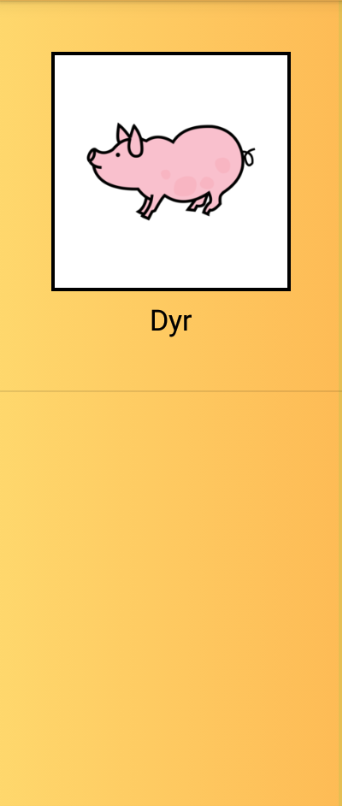
\includegraphics[width=0.25\textwidth]{pictures/application_structure/sidebar}
        \caption{Side bar example}
        \label{fig:side_bar_example}
\end{figure}

\subsection{Bottom bar}
Bottom bars should be entirely contextual and depend on the current content displayed in the current \androidinline{Activity}. A bottom bar should look like Figure \ref{fig:bottom_bar_example}.

\begin{figure}[!htbp]
        \centering
        
\includegraphics[width=0.75\textwidth]{pictures/application_structure/bottombar}
        \caption{Bottom bar example}
        \label{fig:bottom_bar_example}
\end{figure}

\section{Content}
The main content of applications should be in the center of the layout and any menu bars should be above, under, and to the sides of the main content. 

\begin{note}
We recommend using Android \androidinline{Fragment} instances to manage content of an \androidinline{Activity} if the main content of an Android \androidinline{Activity} needs to change between different content that needs to be controlled differently. 
\end{note}